\subsection{Key-Value Store Accelerator}

\begin{figure}
    \label{fig:kvstore}
    \begin{centering}
\includegraphics[width=0.9\linewidth]{../../img/kvstore.pdf}
\caption{Key-Value Store Accelerator}
    \end{centering}
\end{figure}

\subsubsection{Lookup Pipeline}

The main part of the accelerator is a lookup pipeline, which takes keys in
through an input interface and streams out the values through an output
interface. Each interface consists of two decoupled interfaces with ready-valid
signals. The first decoupled interface sends the length of the data to come,
and the second sends the data itself eight bits at a time.

When a key comes into the accelerator, the first thing done is to compute a
primary and secondary hash value. The hash algorithm used is the Pearson
hashing algorithm, a non-cryptographic hashing algorithm implemented as follows.

\begin{verbatim}
    h = array of size n
    for j from 0 to n-1
        h[j] = T[(x[0] + j) & 0xff]
        for i from 1 to length(x) - 1
            h[j] = T[h[j] ^ x[i]]
\end{verbatim}

In this algorithm, \(h\) is one byte in the final hash value,
\(x\) is the message, and \(T\) is a table containing a random permutation of
all the integers from 0 to 255. The outer loop of the algorithm is
parallelized by replicating the following hardware \(n\) times.

\begin{figure}
    \label{fig:hasher}
    \begin{centering}
\includegraphics[width=0.9\linewidth]{../../img/hasher.pdf}
\caption{Hasher}
    \end{centering}
\end{figure}
We use two different tables in order to generate two different hash values,
a primary and a secondary hash. At the same time, we write the key into the
current key memory. When the hasher is finished, it passes these two hashes
to the key comparison unit.

The key comparison unit uses the hash value to index into the key memory.
The key memory reserves 256 bytes for each key, so the starting address of a
key in the memory can be found simply by taking the hash value and shifting it
to the right by a certain number of bits (the shift amount depends on the
word size of the memory, which can be parameterized). Assuming a word size
of eight bits, the algorithm for the key comparison unit would be as follows.

\begin{verbatim}
function keycompare(hash, curKeyLen)
    cmpKeyLen := lenMem(hash)
    if (cmpKeyLen != curKeyLen)
        return false
    for i from 0 to (curKeyLen - 1)
        allInd = (hash << 8) | i
        if (curKeyMem(i) != allKeyMem(allInd))
            return false
    return true
\end{verbatim}

Note that there is also a memory to store the lengths of keys.
The key comparison unit will check the primary hash value and, if that does
not match, the secondary hash value. If one of the two possible keys matches,
the correct hash value is then passed to the value memory unit. The value
memory will then look up the starting address and length of the value from a
table, and begin streaming out the value through the output interface.
If neither of the two keys matched, the value memory unit will send
a zero through the length interface to indicate that no value was found.

The interfaces between subsequent pipeline stages (hashing, key comparison,
and value streaming) are constructed so that all three stages can operate
simultaneously. That way, the accelerator can process three in-flight keys
at a time. Tags are used to allow external hardware to determine which
response corresponds to which key. The one complication in decoupling the
pipeline stages is that both the hasher/writer stage and the key comparison
stage access the current key memory. This problem is solved by doubling the
key memory. The writer writes to one half of the memory while the key
comparison unit reads from the other half. When both units finish processing
a key, they switch halves so that the key comparison unit reads the key which
was just written and the writer overwrites the key which was just processed.

\subsubsection{Control through RoCC interface}

The accelerator is configured from software through the RoCC command interface.
To place a key into the accelerator, the lookup pipeline must first be
placed into write mode. In this mode, the hasher will no longer take keys
from the traffic manager, but will instead take the key from the memory handler,
which reads in the keys from DRAM through the RoCC memory interface.

Once the key is read in and hash values computed, the key compare unit will
then determine which hash slot the key can be placed in. A key can be placed
in a hash slot if the slot is empty, the key in the slot is the same as the
key to be placed, or the key has a lower weight than the key being placed.
The weight is simply a saturating count of how frequently the key is accessed.
The count can be reset from software so that keys which were once popular but
are no longer can be evicted.

Once the lookup pipeline has determined where the new key can be placed, the
controller will instruct the memory handler to read the value through the
RoCC memory interface and write it into the value memory.
